\definecolor{myblue}{RGB}{0,102,204}
\definecolor{myorange}{RGB}{255,153,51}

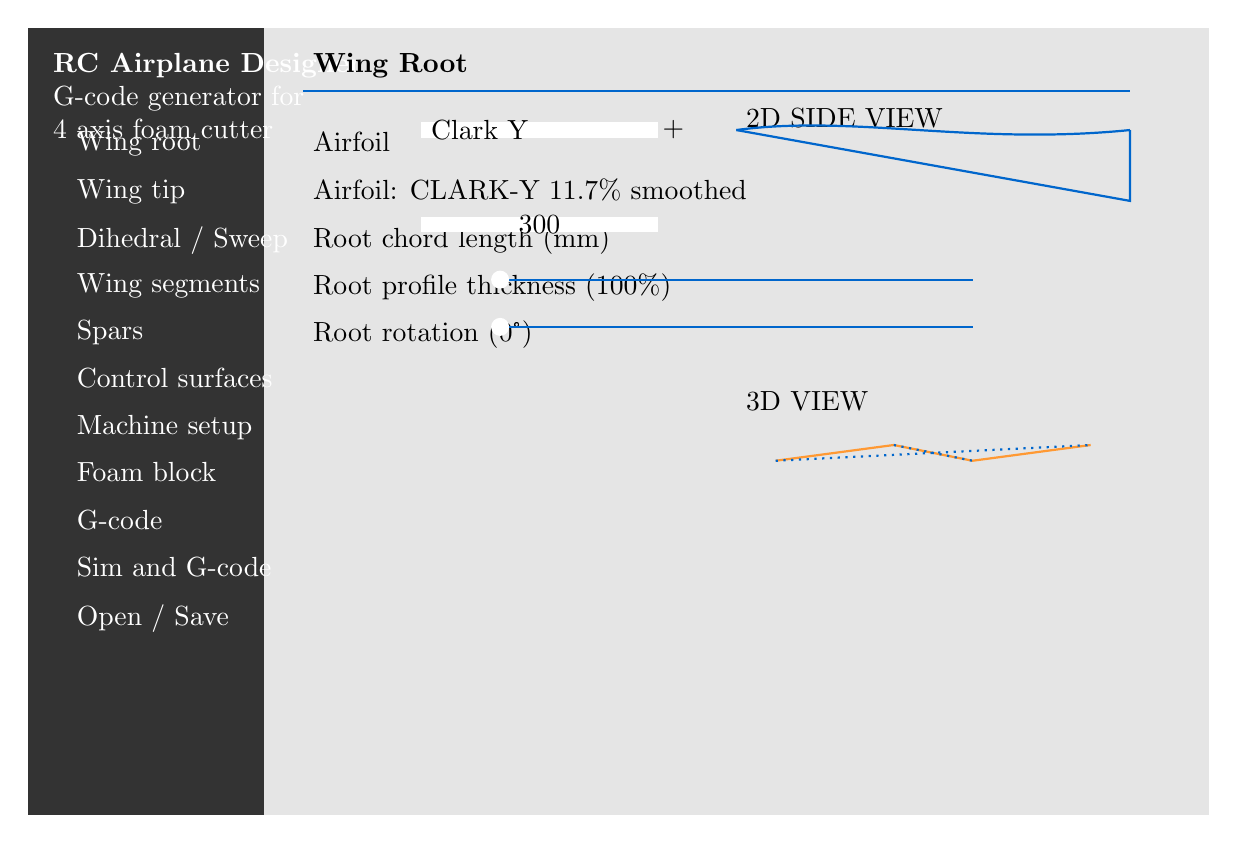
\begin{tikzpicture}
	
	\fill[gray!20] (0,0) rectangle (15,-10);
	
	\fill[black!80] (0,0) rectangle (3,-10);
	
	\node[text=white, anchor=north west, align=left] at (0.2,-0.2) {
		\textbf{RC Airplane Designer}\\
		G-code generator for\\
		4 axis foam cutter
	};
	
	\node[text=white, anchor=north west] at (0.5,-1.2) {Wing root};
	\node[text=white, anchor=north west] at (0.5,-1.8) {Wing tip};
	\node[text=white, anchor=north west] at (0.5,-2.4) {Dihedral / Sweep};
	\node[text=white, anchor=north west] at (0.5,-3.0) {Wing segments};
	\node[text=white, anchor=north west] at (0.5,-3.6) {Spars};
	\node[text=white, anchor=north west] at (0.5,-4.2) {Control surfaces};
	\node[text=white, anchor=north west] at (0.5,-4.8) {Machine setup};
	\node[text=white, anchor=north west] at (0.5,-5.4) {Foam block};
	\node[text=white, anchor=north west] at (0.5,-6.0) {G-code};
	\node[text=white, anchor=north west] at (0.5,-6.6) {Sim and G-code};
	\node[text=white, anchor=north west] at (0.5,-7.2) {Open / Save};
	
	\node[anchor=north west, align=left] at (3.5,-0.2) {\textbf{Wing Root}};
	\draw[myblue, thick] (3.5,-0.8) -- (14,-0.8);
	
	\node[anchor=north west] at (3.5,-1.2) {Airfoil};
	\fill[white] (5,-1.4) rectangle (8,-1.2);
	\node[right] at (5,-1.3) {Clark Y};
	\node at (8.2,-1.3) {+};
	
	\node[anchor=north west] at (3.5,-1.8) {Airfoil: CLARK-Y 11.7\% smoothed};
	
	\node[anchor=north west] at (3.5,-2.4) {Root chord length (mm)};
	\fill[white] (5,-2.6) rectangle (8,-2.4);
	\node at (6.5,-2.5) {300};
	
	\node[anchor=north west] at (3.5,-3.0) {Root profile thickness (100\%)};
	\draw[myblue, thick] (6,-3.2) -- (12,-3.2);
	\draw[white, thick, fill=white] (6,-3.2) circle (0.1);
	
	\node[anchor=north west] at (3.5,-3.6) {Root rotation (0\textdegree)};
	\draw[myblue, thick] (6,-3.8) -- (12,-3.8);
	\draw[white, thick, fill=white] (6,-3.8) circle (0.1);
	
	\node[anchor=north west] at (9,-0.9) {2D SIDE VIEW};
	\draw[myblue, thick] (9,-1.3) .. controls (10.5,-1.1) and (12,-1.5) .. (14,-1.3);
	\draw[myblue, thick] (9,-1.3) -- (14,-2.2) -- (14,-1.3);
	
	\node[anchor=north west] at (9,-4.5) {3D VIEW};
	\draw[myorange, thick] (9.5,-5.5) -- (11,-5.3) -- (12,-5.5) -- (13.5,-5.3);
	\draw[myblue, thick, dotted] (9.5,-5.5) -- (13.5,-5.3);
	\draw[myblue, thick, dotted] (11,-5.3) -- (12,-5.5);
	
\end{tikzpicture}